% Build with xetex.
\documentclass[aspectratio=169,handout,bigger]{beamer}

%% -------------------------------------------------------------------------- %%

\usepackage{xunicode}
\usepackage{xltxtra}
\usepackage{graphicx}

\usepackage{color}

\usepackage{setspace}
\usepackage{ragged2e}

\usepackage[normalem]{ulem}

\usepackage{minted}

\usepackage{tikz}
\usetikzlibrary{shapes,arrows,chains,calc,fit,matrix}

%% -------------------------------------------------------------------------- %%

\usepackage{polyglossia}
\setmainlanguage{russian}
\setotherlanguage{english}

% NB: To get MS fonts for OS X:
%
% 1) Install MS Open XML Converter.
% 2) Install OpenXML_all_fonts.pkg from inside of Converter's mpkg.
%
% http://www.labnol.org/software/tutorials/\
% free-download-calibri-font-on-mac/3684/

\setmainfont{Calibri}
\setsansfont{Calibri}
\setmonofont{Consolas}

%% -------------------------------------------------------------------------- %%

\mode<presentation>{
  \usetheme{default}
}

\useinnertheme{circles}

\setbeamertemplate{navigation symbols}{}
\setbeamertemplate{section in toc}[sections numbered]

\definecolor{chart11}{RGB}{0, 0, 0}
\setbeamercolor{title}{fg=chart11}
\setbeamercolor{author}{fg=chart11}
\setbeamercolor{frametitle}{fg=chart11}
\setbeamercolor{itemize item}{fg=chart11}
\setbeamercolor{itemize subitem}{fg=chart11}
\setbeamercolor{itemize subsubitem}{fg=chart11}
\setbeamercolor{section in toc}{fg=chart11}

\setbeamersize{text margin left=0.5cm,text margin right=0.5cm}

%% -------------------------------------------------------------------------- %%

\defbeamertemplate{footline}{left page number}
{%
  \hfill
  \usebeamercolor[fg]{page number in head/foot}%
  \usebeamerfont{page number in head/foot}%
  \insertpagenumber\,/\,\insertpresentationendpage%
  \hspace*{1em}
  \vskip1em%
}
\setbeamertemplate{footline}[left page number]

%% ========================================================================== %%

\title{
\includegraphics[height=.15\textheight]{logo}}
\author{Быстрое прототипирование функциональных макетов UI\\на Lua и Mermaid.js}
\institute{Александр Гладыш\\@agladysh}
\date{Lua in Moscow / DevConf 2017}

%% ========================================================================== %%

\begin{document}

% Using [plain] to avoid frame number on the title page.
\begin{frame}[plain]
 \titlepage
\end{frame}

%% ========================================================================== %%

\begin{frame}{План}

\tableofcontents

\end{frame}

%% ========================================================================== %%

\section*{}

\begin{frame}{Обо мне}

\begin{itemize}
\item Программист
\item Сейчас основном занимаюсь управлением
\item Пишу на Lua с 2005-го года
\end{itemize}

\end{frame}

%% ========================================================================== %%
\section{Кейс}
%% ========================================================================== %%

\begin{frame}{Кейс}
  \begin{itemize}
    \item Огромная профессиональная энтерпрайз-система
    \item обновляется от 20-летнего приложения для Windows
    \item до современного одностраничного веб-приложения.
  \end{itemize}
\end{frame}

%% -------------------------------------------------------------------------- %%

\begin{frame}{Система огромна}
  Ни один человек не в состоянии при проектировании принять обоснованное решение
  по сложному вопросу в одиночку

  \begin{itemize}
    \item У экспертов в технологии нет видения нового продукта в целом
    \item ПМ и ПО не рисуют профессионально
          и у них не всегда есть действительно глубокое понимания
          аспектов технологии
    \item Дизайнер имеет лишь поверхностное понимание технологии
  \end{itemize}
\end{frame}

%% -------------------------------------------------------------------------- %%

\begin{frame}{Процесс проектирования и дизайна UI}
  Для каждого "экрана" в приложении:

  \begin{itemize}
    \item Концепция
    \item Функциональные макеты и (иногда) интерактивные эскизы
    \item Дизайн-макеты
    \item Вёрстка
    \item Реализация бизнес-логики
  \end{itemize}
\end{frame}

%% -------------------------------------------------------------------------- %%

\begin{frame}{Функциональный макет}
  Что должно находиться на экране, как это будет РАБОТАТЬ?

  \centering{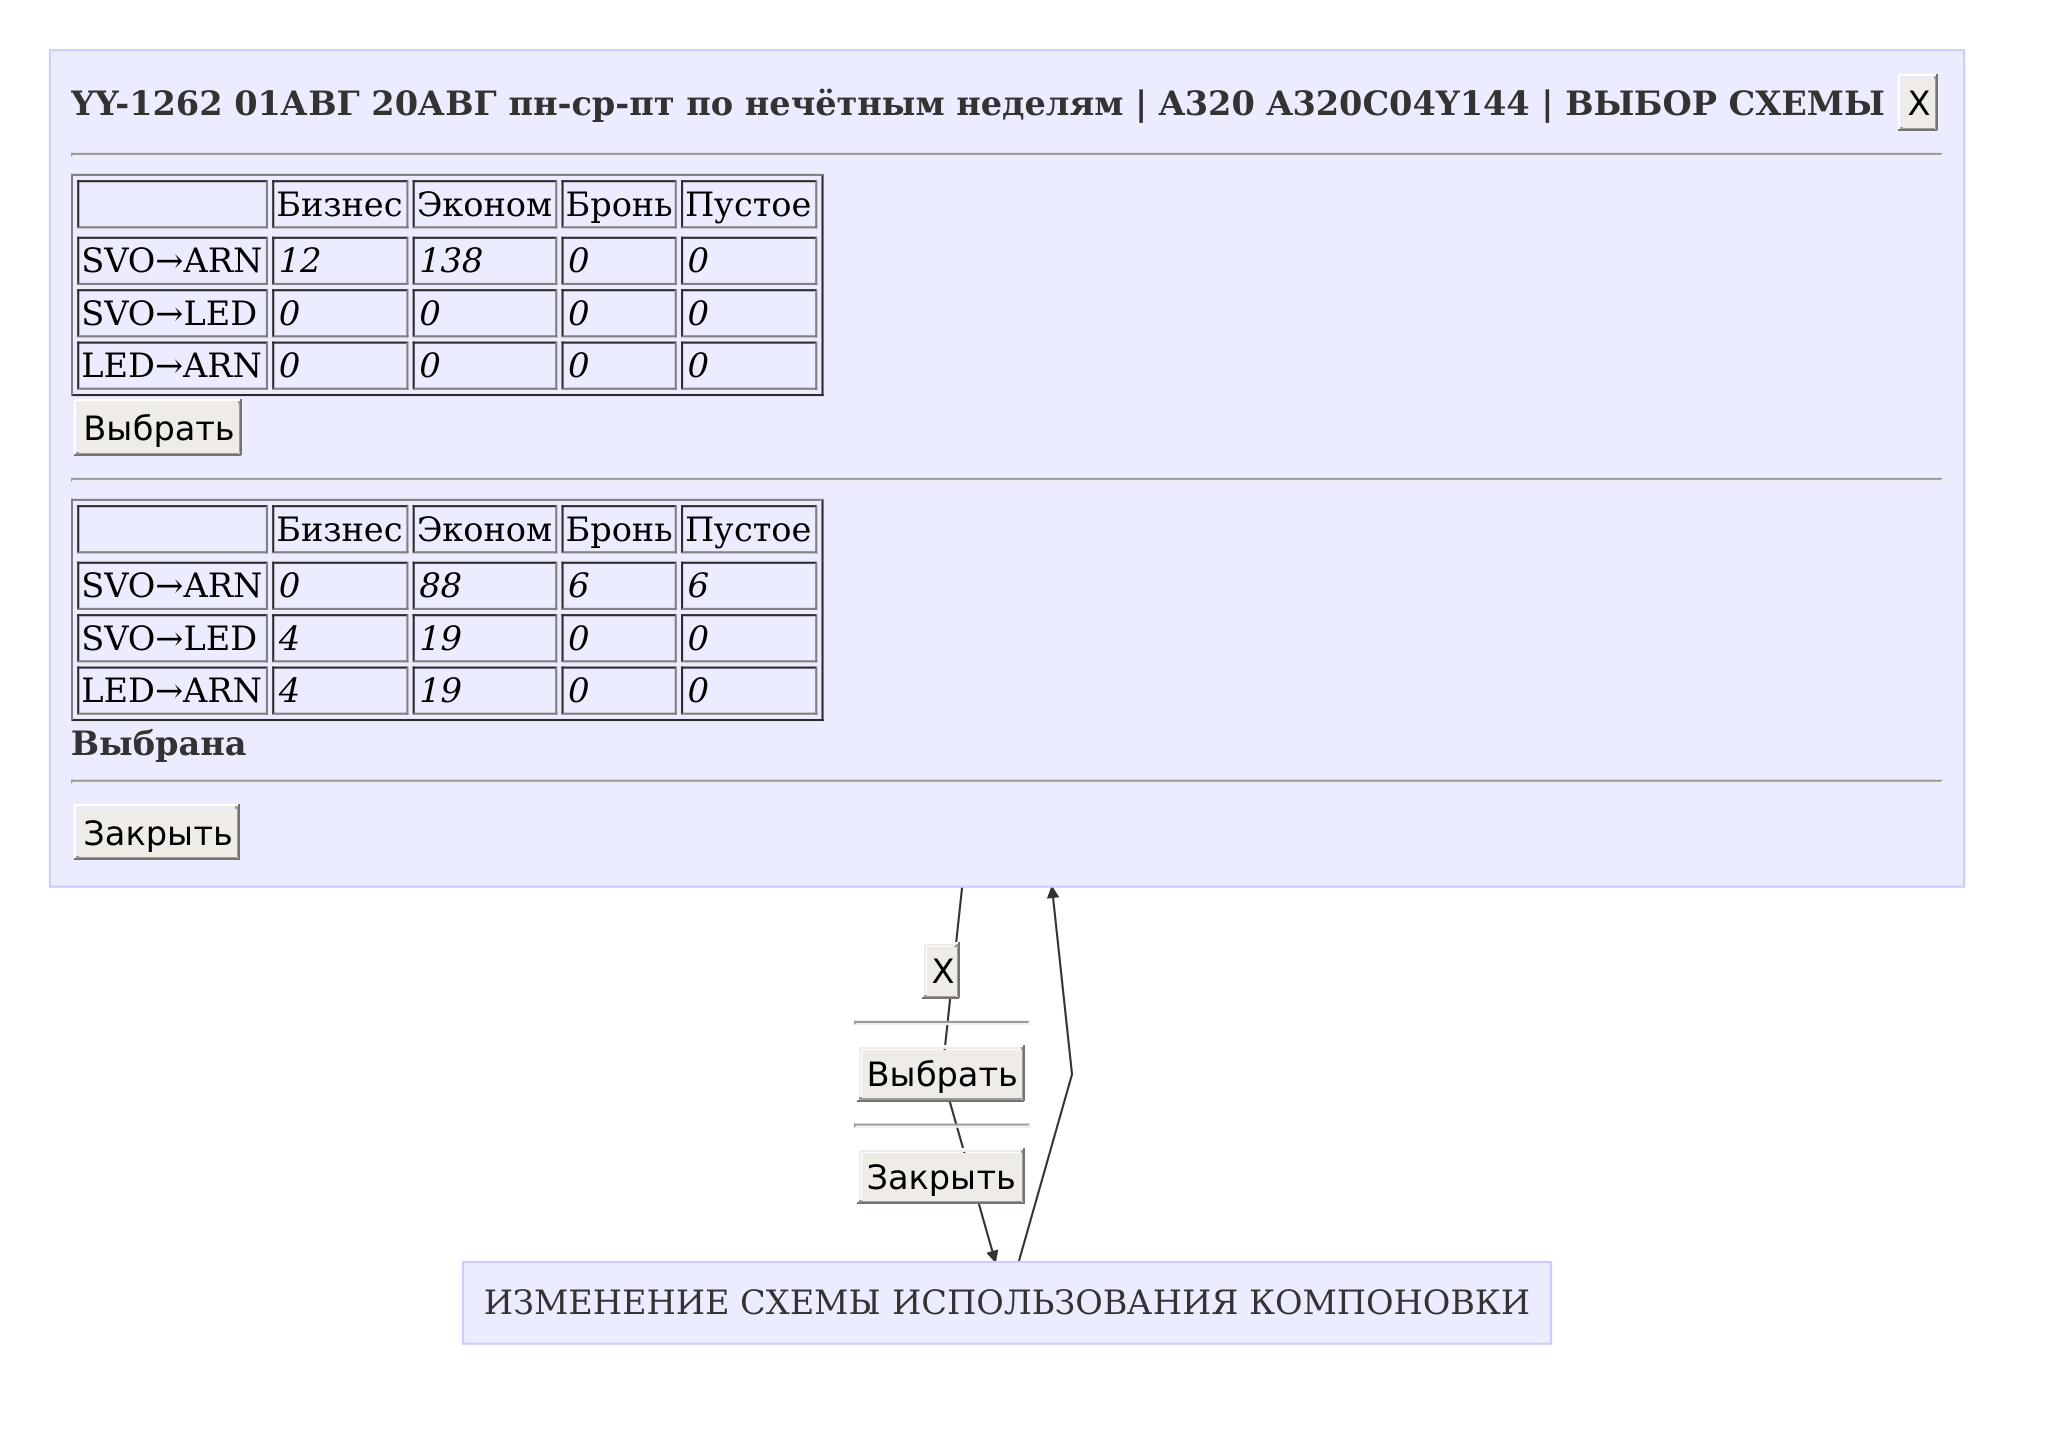
\includegraphics[height=.75\textheight]{seatmap}}
\end{frame}

%% -------------------------------------------------------------------------- %%

\begin{frame}{Дизайн-макет}
  Как это должно ВЫГЛЯДЕТЬ?

  \centering{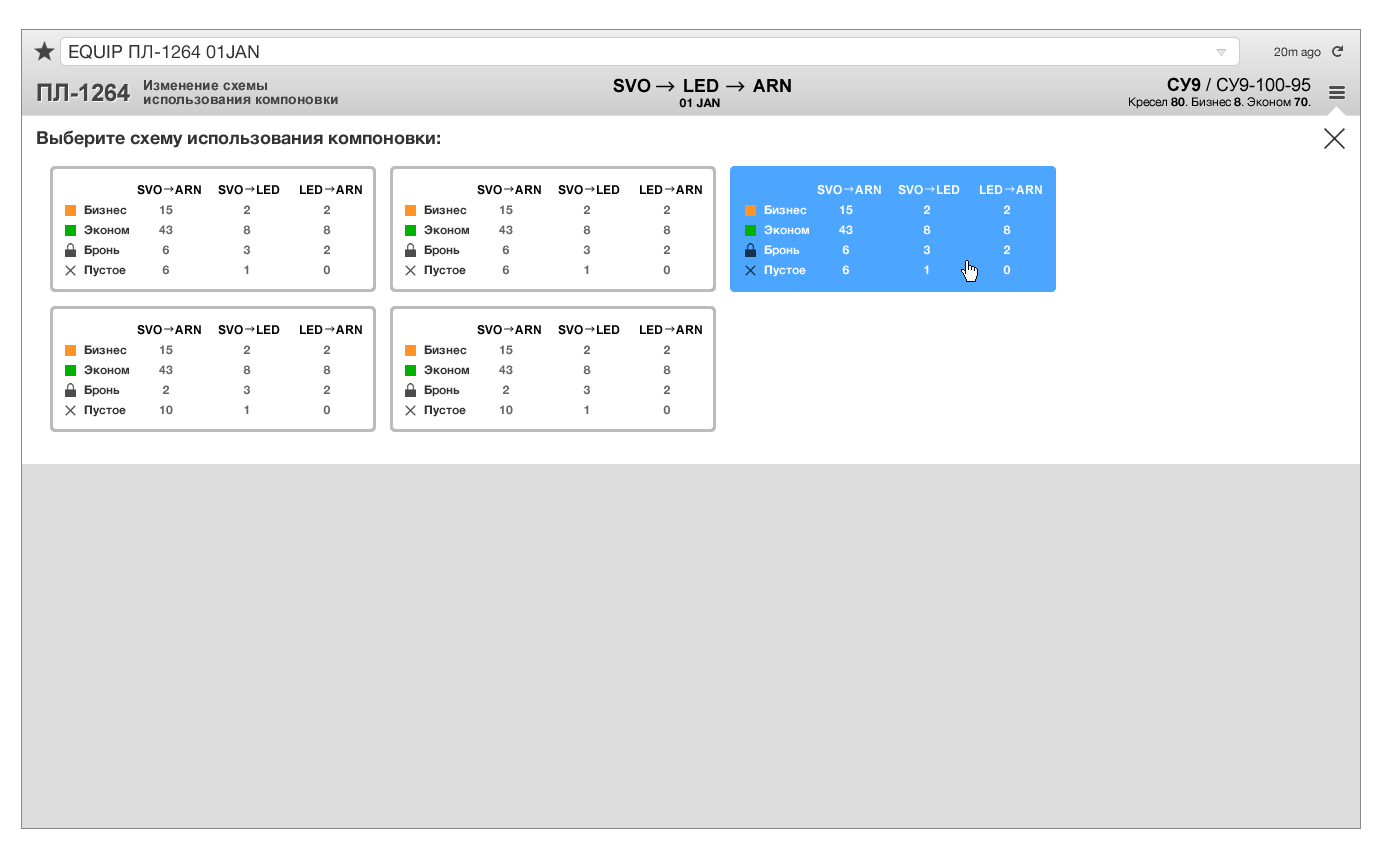
\includegraphics[height=.75\textheight]{EQUIP-1_2}}
\end{frame}

%% -------------------------------------------------------------------------- %%

\begin{frame}{Задачи}
  \begin{itemize}
    \item Нужна диаграмма переходов между экранами приложения.
    \item Нужны функциональные макеты самих экранов.
    \item В принципе не важно как я получу эту диаграмму и макеты,
          до тех пор пока их легко сделать и изменить
          и есть хоть какие-то механизмы для повторного использования наработок.
  \end{itemize}
\end{frame}

%% ========================================================================== %%
\section{Подходы к проектированию}
%% ========================================================================== %%

\begin{frame}{Инструменты}
  \begin{itemize}
    \item Photoshop (Krita, Gimp...)
    \item InkScape
    \item Google Documents
    \item Visio
    \item Balsamiq
    \item Sketch
    \item ...
  \end{itemize}
  \vskip 1em
  Я --- программист.
  Мне легче работать со структурированным текстом чем с изображениями.
  \vskip 1em
  Быстрее всего я работаю с клавиатурой, не трогая мышь.
\end{frame}

%% ========================================================================== %%
\section{Enter the Mermaid}
%% ========================================================================== %%

\begin{frame}{Enter the Mermaid}
  http://bit.ly/mermaid-editor

  \centering{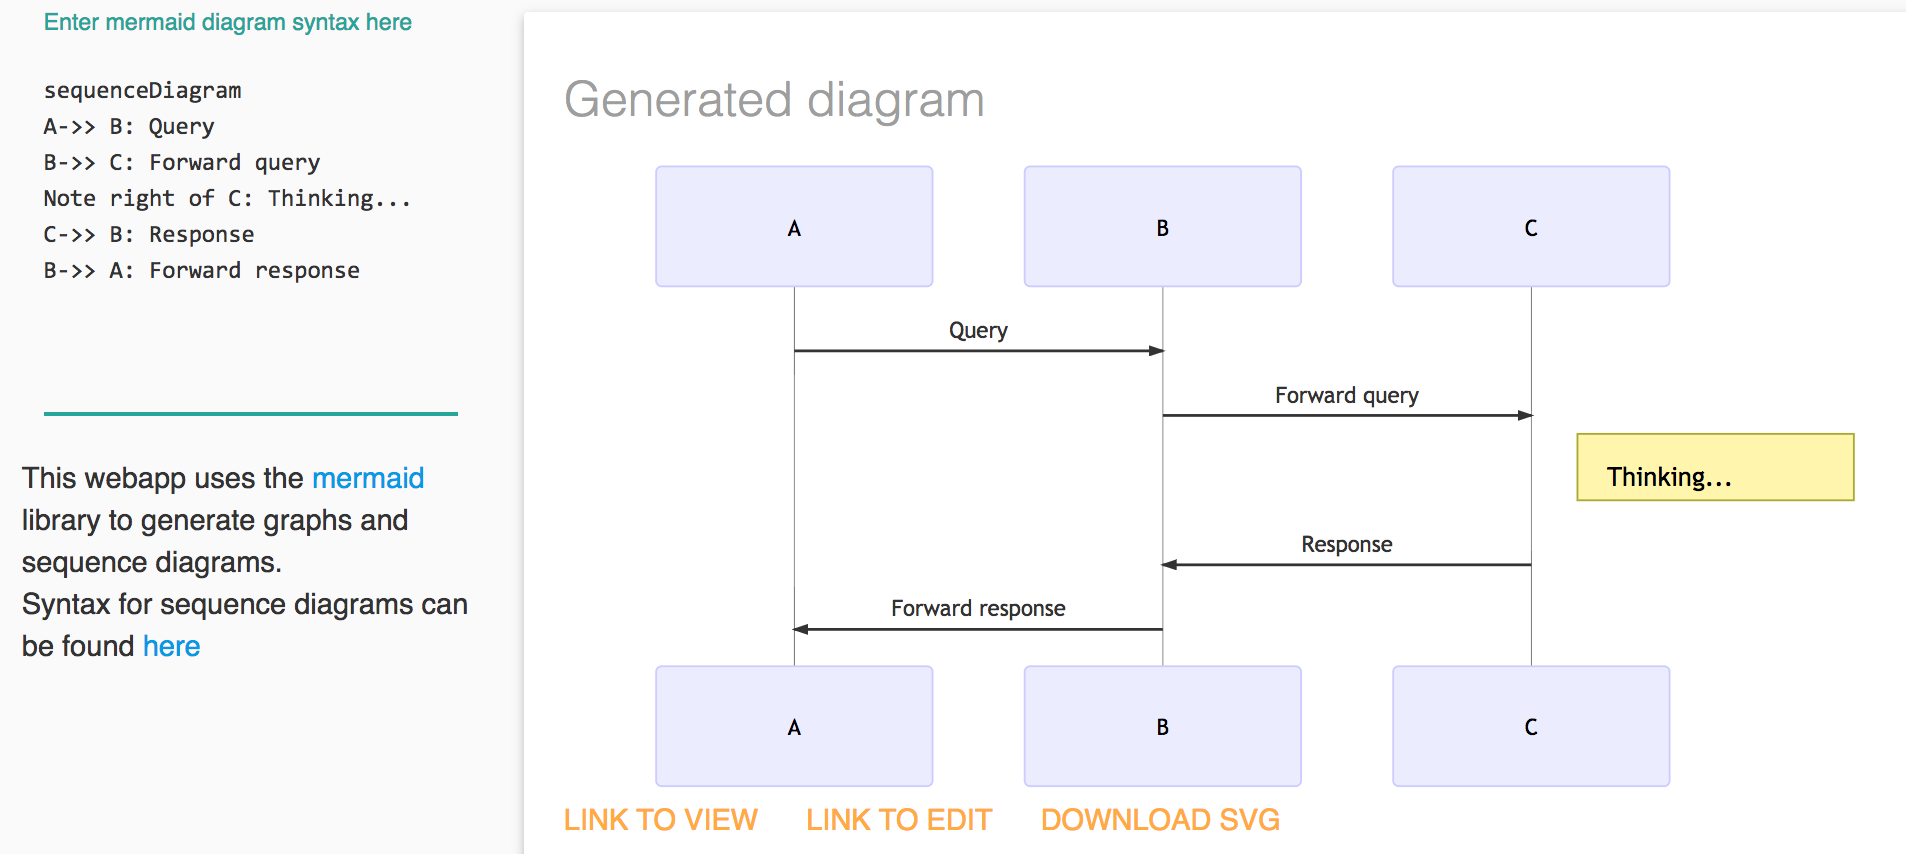
\includegraphics[width=.95\textwidth]{liveeditor}}
\end{frame}

%% -------------------------------------------------------------------------- %%

\begin{frame}[fragile]{Диаграмма переходов между экранами}
  \begin{columns}
    \begin{column}{.5\textwidth}
\begin{minted}{text}
graph TD

list[List of Flights]
new[New Flight Form]

list-->|Create|new
\end{minted}
\end{column}
\begin{column}{.5\textwidth}
\centering{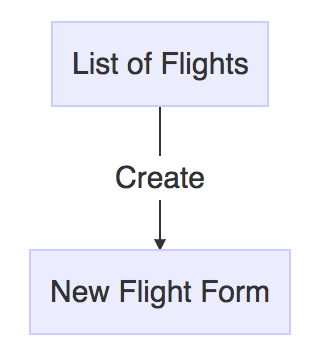
\includegraphics[height=.9\textheight]{flights-1}}
\end{column}
\end{columns}
\end{frame}

%% -------------------------------------------------------------------------- %%

\begin{frame}[fragile]{Диаграма переходов между экранами (II)}
  \begin{columns}
    \begin{column}{.5\textwidth}
\begin{minted}{html}
graph TD

list[List of Flights]
new[New Flight Form]

list-->|"
<button>Create</button>
"|new
\end{minted}
\end{column}
\begin{column}{.5\textwidth}
\centering{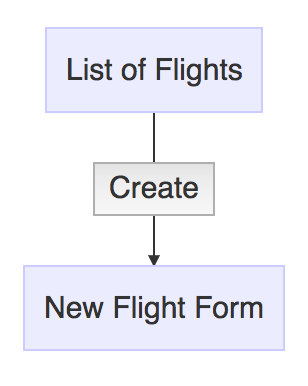
\includegraphics[height=.9\textheight]{flights-2}}
\end{column}
\end{columns}
\end{frame}

%% -------------------------------------------------------------------------- %%

\begin{frame}[fragile]{Функциональные макеты экранов}
  \begin{columns}
    \begin{column}{.5\textwidth}
\begin{minted}{text}
graph TD

list["<b>List of Flights</b>
    <hr>
    <i>(No flights)</i><hr>
    <button>Create</button>"]

new["New Flight Form"]
list-->|"
<button>Create</button>
"|new
\end{minted}
  \end{column}
  \begin{column}{.5\textwidth}
    \centering{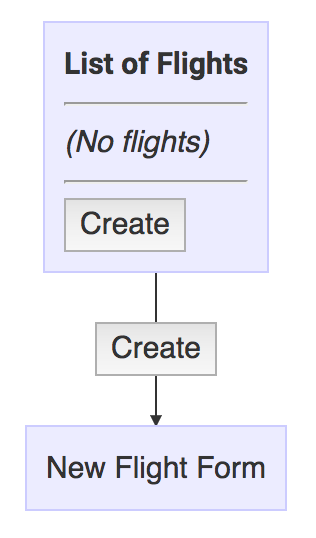
\includegraphics[height=.9\textheight]{flights-3}}
  \end{column}
  \end{columns}
\end{frame}

%% -------------------------------------------------------------------------- %%

\begin{frame}[fragile]{Функциональные макеты экранов (II)}
  \begin{columns}
    \begin{column}{.6\textwidth}
\begin{minted}{text}
graph TD
list["List of Flights"]
new["<b>New Flight</b><hr>
<input value='SU' size='2'>-
<input value='2618' size='4'><br>
<input value='MOW' size='5'> to
<input value='BRU' size='5'><br>
<input value='20:50' size='5'> to
<input value='22:30' size='5'>
<hr><button>Create</button>
<u>Cancel</u>"]
new-->|"
<button>Create</button>"|list
new-->|"<u>Cancel</u>"|list
\end{minted}
    \end{column}
    \begin{column}{.3\textwidth}
      \centering{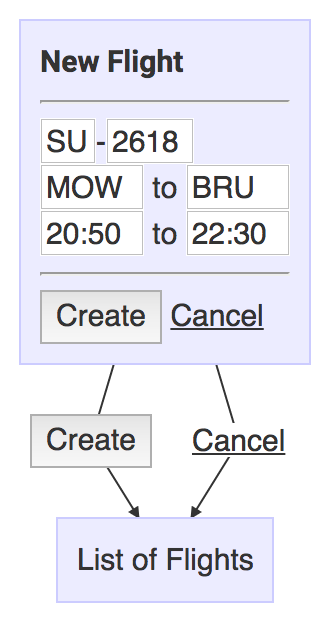
\includegraphics[height=.9\textheight]{flights-4}}
    \end{column}
  \end{columns}
\end{frame}

%% -------------------------------------------------------------------------- %%

\begin{frame}{Результаты}
  \centering{
    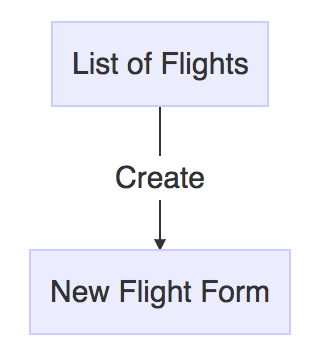
\includegraphics[width=.28\textwidth]{flights-1}
    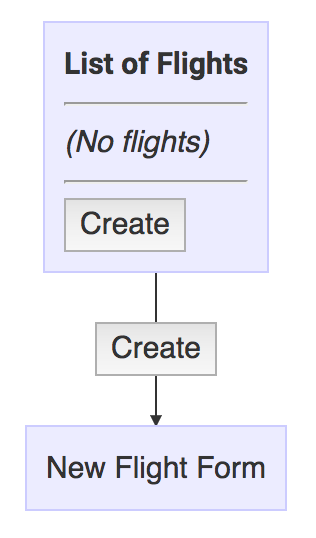
\includegraphics[width=.28\textwidth]{flights-3}
    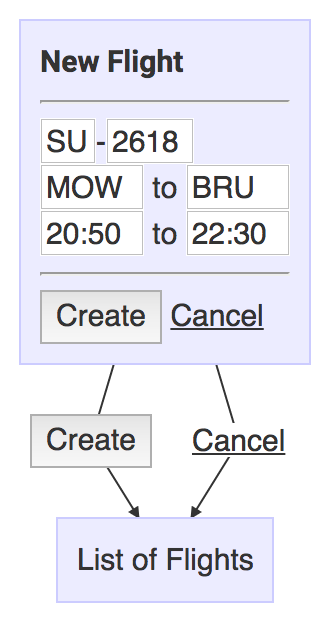
\includegraphics[width=.28\textwidth]{flights-4}
  }
\end{frame}

%% -------------------------------------------------------------------------- %%

\begin{frame}[fragile]{Без шаблонов тяжко: list}
\begin{minted}{text}
<b>${title List of Flights}</b><hr>

<i>(No flights)</i><hr>

${link new <button>Create</button>}
\end{minted}
\end{frame}

%% -------------------------------------------------------------------------- %%

\begin{frame}[fragile]{Без шаблонов тяжко: new}
\begin{minted}{text}
<b>${title New Flight}</b><hr>

<input value='SU' size='2'>-
<input value='2618' size='4'><br>

<input value='MOW' size='4'> to
<input value='BRU' size='4'><br>

<input value='20:50' size='5'> to
<input value='10:30' size='5'><hr>

${link list <button>Create</button>}
${link list <button>Cancel</button>}
\end{minted}
\end{frame}

%% ========================================================================== %%
\section{Шаблоны Lugram}
%% ========================================================================== %%

\begin{frame}[fragile]{Базовые хелперы}
\begin{minted}{text}
${title New Flight}
\end{minted}

  \${title <text:*>}

  \vskip 1em

\begin{minted}{text}
${link list <button>Create</button>}
\end{minted}

  \${link <screen:word> <body:*>}
\end{frame}

%% -------------------------------------------------------------------------- %%

\begin{frame}[fragile]{Базовые хелперы: pass-through макросы}
\begin{minted}{text}
${define title {{'*', 'text'}} [[${text}]]}

${title New Flight} --> New Flight
\end{minted}

\vskip 1em

\begin{minted}{text}
${define link
  {{'word', 'target'}, {'*', 'body'}}
  [[${body}]]}

${link list <button>Create</button>}
--> <button>Create</button>
\end{minted}

\vskip 1em

\${define <symbol:word> <arguments:table> <code:*>}
\end{frame}

%% -------------------------------------------------------------------------- %%

\begin{frame}[fragile]{define}
\begin{minted}{lua}
define = function(context, str)
  local symbol, str = eat.word(str)
  local args, str = eat.table(str)
  local code, str = eat['*'](str)
  args, code = lua_value(args), lua_value(code)
  if type(code) == 'string' then code =
    function(ctx) return ctx:replace(code) end
  end
  context._ROOT[symbol] = function(parent, str)
    local ctx = { }
    for i = 1, #args do
      ctx[args[i][1]], str = eat[args[i][2]](str)
    end
    return code(parent:push(ctx))
  end
end
\end{minted}
\end{frame}

%% -------------------------------------------------------------------------- %%

\begin{frame}[fragile]{Хелперы: код на Lua}
\begin{minted}{text}
${define title {{'*', 'text'}} function(context)
  local text = context:replace(context.text)
  context._ROOT._SCREENS[text] = text
  return text
end}
\end{minted}

\begin{minted}{text}
${define link {{'word', 'target'}, {'*', 'body'}}
function(context)
  local target = context:replace(context.text)
  context._ROOT._LINKS[target] = context._MODULE
  context:include(target) -- Ignoring result
  return context:replace(context.body)
end}
\end{minted}
\end{frame}

%% -------------------------------------------------------------------------- %%

\begin{frame}[fragile]{include}
\begin{minted}{lua}
include = function(context, template)
  return context:push(
    { _MODULE = template }
  ):replace(
    assert(io.open(filename)):read("*a")
  )
end
\end{minted}
\end{frame}

%% -------------------------------------------------------------------------- %%

\begin{frame}{Виды диаграмм}
  В зависимости от того, как определить \${title} and \${link},
  можно получить несколько видов диаграмм из одного набора шаблонов:

  \begin{itemize}
    \item Outline (только заголовки и стрелки, "переходы между экранами")
    \item Closeup (содержимое "текущего" экрана и переходы из него в другие экраны)
    \item Printable (только содержимое "текущего" экрана)
  \end{itemize}
\end{frame}

%% -------------------------------------------------------------------------- %%

\begin{frame}[fragile]{Некоторые другие полезные хелперы}
\begin{minted}{text}
${define # {{'*', 'comment'}} [[]]}
${define --[HR]------...--------- {} [[<hr>]]}

${define expr {{'*', 'code'}} function(context)
  return assert(loadstring('return '
    .. context:replace(context.code)))()
end}
\end{minted}
\end{frame}

%% -------------------------------------------------------------------------- %%

\begin{frame}[fragile]{Хелпер with}
\begin{minted}{text}
${define with {{'table', 'more_context'},
  {'*', 'body'}} function(context)
  return context:replace(
    context:push(context.more_context),
    context.body)
end}

${define form {} [[
  ${when editable
    <input value='MOW'> to <input value='BRU'>}
  ${unless editable MOW to BRU}
]]}

${with {editable = true} ${form}}
\end{minted}
\end{frame}

%% -------------------------------------------------------------------------- %%

\begin{frame}[fragile]{Хелпер with (II)}
\begin{minted}{html}
${define histogram {{'word', 'a'},
  {'word', 'b'}, {'word', 'c'}} [[
${with { w = '${expr ${a} + ${b} + {c}}' }
  <div style='width:${w}px' class='red'>
    <div style='width:${a}px'
      class='green'>${a}</div>
    <div style='width:${b}px'
      class='blue'>${b}</div>
  </div>
}]]}

${histogram 1 2 3}
\end{minted}
\end{frame}

%% ========================================================================== %%
\section{В завершение}
%% ========================================================================== %%

\begin{frame}{Немного статистики}
  \begin{itemize}
    \item Ядро примерно в 250 строк было написано за два дня.
    \item После шести месяцев нефуллтайм использования ядро выросло
          примерно до 330 строк кода. В основном была добавлена диагностика.
    \item Разработано порядка 60 макетов (5 тысяч строк кода шаблонов),
          будет ещё больше.
  \end{itemize}
\end{frame}

%% -------------------------------------------------------------------------- %%

\begin{frame}{Стоит ли овчинка выделки?}
  Да.
  \begin{itemize}
    \item Получился дешёвый легковесный и гибкий фреймворк
          для разработки функциональных макетов,
          с которым мне лично легко работать.
    \item Выдача этого фреймворка, хотя и не идеальна,
          вполне доступна для понимания всеми членами команды.
    \item (И было прикольно написать ещё один шаблонизатор!)
  \end{itemize}
\end{frame}

%% -------------------------------------------------------------------------- %%

\begin{frame}{Почему не X?}
  \begin{itemize}
    \item Разработка Lugram потребовала настолько мало усилий,
          что адаптация существующего инструмента под мои нужды
          (или даже просто его освоение), вероятно,
          стоили было бы столько же или больше.
    \item Но если вы знаете подходящий инструмент --- делитесь!
  \end{itemize}
\end{frame}

%% -------------------------------------------------------------------------- %%

\begin{frame}{Проблемы}
  \begin{itemize}
    \item Диагностика ошибок и отладка.
          В данный момент почти полностью отсутствуют.
          Небольшими усилиями можно добиться значительных улучшений.
    \item Отладка отрисовки HTML. Сложно как в IE6. Очень сложно улучшить.
          Нужно следить за тем, чтобы HTML выходил максимально простым.
    \item Можно расширить выразительные возможности языка.
          Но имеющихся пока вполне достаточно.
  \end{itemize}
\end{frame}

%% ========================================================================== %%

\section{Вопросы?}

%% ========================================================================== %%

% Using [plain] to hide frame number.
\begin{frame}[plain]{Вопросы?}

\begin{center}
\Huge{@agladysh}
\end{center}

\begin{center}
\Large{agladysh@gmail.com}
\end{center}

\begin{center}
https://github.com/tais-aero/lugram
\end{center}

\end{frame}

%% ========================================================================== %%

\end{document}

% Пропорции слайда
% Логотип девконфа на слайдах
